\documentclass[letterpaper]{article}

% used for unnumbered equations
\usepackage{amsmath}
% used for enumerating problem parts by letter
\usepackage{enumerate}
% used for margins
\usepackage[letterpaper,left=1.25in,right=1.25in,top=1in,bottom=1in]{geometry}
% used for header and page numbers
\usepackage{fancyhdr}
% used for inserting images
\usepackage{graphicx}
% used for preventing paragraph indentation
\usepackage[parfill]{parskip}
% used for section formatting as problem
\usepackage[explicit]{titlesec}
% used for side-by-side images in a figure
\usepackage{subcaption}

\graphicspath{ {images/} }
\pagestyle{fancy}
\fancyfoot{}
% header/footer settings
\lhead{Kevin Nash}
\chead{EECS 325 -- Homework 4}
\rhead{\today}
\cfoot{\thepage}

\titleformat{\section}{\normalfont\large\bfseries}{}{0em}{#1\ \thesection}
\newcommand{\problem}{\section{Problem}}
\newcommand{\bparts}{\begin{enumerate}[(a)]}
\newcommand{\eparts}{\end{enumerate}}

\begin{document}

\problem{}
\bparts
\item
TCP is operating in slow start over transmission rounds 1--6 and 23--26.

These slow start intervals can be identified by their initial congestion
windows, which have a size of one segment, as well as the window's exponential
increase following the first transmission round of each interval.
\item
TCP is operating in congestion avoidance over transmission rounds 6--22.

This congestion avoidance interval can be identified by the window's additive
increases and multiplicative decreases over the interval.
\item
After transmission round 16, segment loss is detected by a triple duplicate
packet because the window size is reduced multiplicatively, not reset
altogether, as is the case following a timeout.
\item
After transmission round 22, segment loss is detected by a timeout because
the window size is reset to 1 segment, as is the case following a timeout.
\item
The initial value of \texttt{sstresh} is 32: the apparent window size
when TCP transitions from slow start to congestion avoidance.
\item
The value of \texttt{ssthresh} at transmission round 18 is 21: half the
window size at transmission round 16, in which segment loss occurs.
\item
The value of \texttt{ssthresh} at transmission round 24 is 14: half
(floored) the window size at transmission round 22, in which segment loss occurs.
\item
The 70th segment is sent during transmission round 7.

The transmission round at which the $N$th segment is sent can be found by
summing the window size at increasing transmission rounds until $N$ is met
or exceeded.

In this case, $\sum_{i=1}^6{TR_i}=63$ and $\sum_{i=1}^7{TR_i}=96$.
\item
If a packet loss is detected after transmission round 26 by the receipt of
a triple duplicate ACK, \texttt{ssthresh} will be set to 4: half the window
size at transmission round 26. The window will then be set to 7: three
segments greater than the threshold, to match the graph's previous segment
loss results.
\eparts

\problem{}
The maximum amount of data on the link is
\begin{equation*}
bandwidth \times RTT \Rightarrow 100\ \mathrm{Mbps} \times 100\ \mathrm{ms}
= 10\ \mathrm{Mb} = 1 \times 10^7\ \mathrm{bits}
\end{equation*}
The minimum number of bits in the window required to represent 10,000,000
is 21. 20 is too few, as \mbox{$2^{20}=1,048,576$}.

The number of bits in the sequence number field must be great enough to
contain the entire segment. We are told that the maximum segment lifetime
is 60 seconds. Therefore in the lifetime
\begin{equation*}
100\ \mathrm{Mbps} \times 60\ \mathrm{s} = 6,000\ \mathrm{Mb} = 6 \times 10^9
\ \mathrm{bits}
\end{equation*}
The minimum number of bits in the sequence number field required to represent
$6 \times 10^9$ is 33. 32 is too few, as \mbox{$2^{32} \approx 4.3 \times 10^9$}.

\problem{}
\textit{Note: this answer is based on the diagram on Lecture 13, Slide 3}.\\
A congestion control that uses additive increase and additive decrease in
equal measure, as the problem describes, will be fair by virtue of having
a $1:1$ ratio of increases and decreases. In the left figure we observe
that the increases and decreases maintain a line parallel to the line
representing equal bandwidth share. In the right figure we observe that
if the ratio is not fair to both connections, a kind of drift occurs.
\begin{figure}
\begin{subfigure}{.5\textwidth}
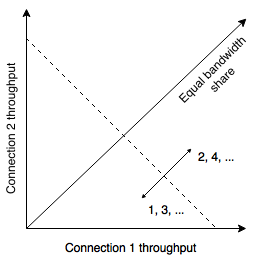
\includegraphics[scale=0.75]{diagram1}
\end{subfigure}
\begin{subfigure}{.5\textwidth}
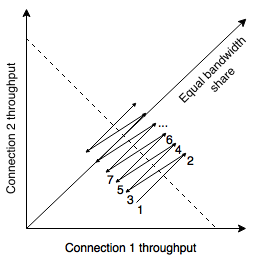
\includegraphics[scale=0.75]{diagram2}
\end{subfigure}
\end{figure}


\problem{}
We are told that TCP inherits ideas from both GBN and SR. Using SR, the number
of distinct sequence numbers must be at least $2N$. TCP
suffers a similar drawback as SR: when ACKs are not received by the sender,
the reciever's window can shift while the sender's does not. Therefore, the
minimum window size should match that of SR: $2N$.

\problem{}
This problem describes a scenario in which an attacker wants to attack a web
server but does not want packets to be traced back to itself, which would
allow the receiver to filter future malicious packets from the attacker.

The attacker can modify its packets before departure so that before it sends
SYN segments to the web server it replaces the sender's address with that of
a ``friendly'' address, such as one within the web server's own IP range.

\problem{}
Throughput is given by
\begin{equation*}
R = I/T
\end{equation*}
$R$ is the rate of transmission, $I$ is the amount transmitted, and
$T$ is the time taken to do so.

First, a handshake, which takes $2 RTT$, occurs. Once that is complete, the
sender has a $1MSS$ window, and thus the sender sends only one segment. The
sender then waits to send following segments until it receives an ACK, which
takes $1 RTT$. Summing the above trips, we get $3 RTT$ before all data is
received.
\begin{equation*}
T = 3RTT = 3 \times 40\ \mathrm{ms}
\end{equation*}
\begin{equation*}
I = 4K\ \ \mathrm{(given)}
\end{equation*}
\begin{equation*}
R = I/T = \frac{4K}{120\ \mathrm{ms}} = 330\ \mathrm{Kbps}
\end{equation*}
\begin{figure}
\centering
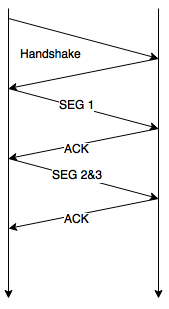
\includegraphics[scale=0.75]{timedia}
\end{figure}

\end{document}
